% Template for PLoS
% Version 1.0 January 2009
%
% To compile to pdf, run:
% latex plos.template
% bibtex plos.template
% latex plos.template
% latex plos.template
% dvipdf plos.template

\documentclass[10pt]{article}

%
%% \usepackage[T1]{fontenc}
%% \usepackage[utf8]{inputenc}
%% \usepackage{xspace}
%% \usepackage{listings}
%% \usepackage{times}
%% \usepackage{subfigure}
%% \usepackage{graphicx}
%% \usepackage{tabularx}
%% \usepackage{natbib}
%% \usepackage{latexsym}
%% \usepackage{color}
%% \usepackage{tikz}
%% \usepackage{amssymb}
%% \usepackage{amsmath}
%% \usepackage{float}
%% \usepackage{textcomp}
%% \usepackage{graphicx}
%% \usepackage{booktabs}
%% \usepackage{url}
%% \usepackage{longtable}
%% \usepackage[figuresright]{rotating}
%% \usepackage{colortbl}
%% \usepackage[noend]{algorithmic}
%% \usepackage[algoruled, vlined, linesnumbered]{algorithm2e}
%% \usepackage{textcomp}

%% \usepackage{rotating}
%% \usepackage{multirow}
%% \usepackage{slashbox}
%% \usepackage{manfnt}
%% \usepackage{skull}
%% \usepackage{wrapfig}

\renewcommand\vec[1]{\boldsymbol{#1}} % vector

\def\bbbr{{\rm I\!R}}
\def\bbbe{{\rm I\!E}}
\newcommand{\R}{{\bbbr}{}}
\newcommand{\E}{{\bbbe}{}}
\newcommand{\actorcritic}{{\scshape Actor-Critic}\xspace}
\newcommand{\mdp}{{\scshape mdp}\xspace}
\newcommand{\mdps}{{\scshape mdp}s\xspace}
\newcommand{\tbn}{{\scshape 2tbn}\xspace}
\newcommand{\tbns}{{\scshape 2tbn}s\xspace}
\newcommand{\td}{{\scshape td}\xspace}
\newcommand{\tdo}{{\scshape td}(0)\xspace}
\newcommand{\tdlambla}{{\scshape td($\lambda$)}\xspace}
\newcommand{\tdlearn}{{\scshape td \mbox{-} learning}\xspace}
\newcommand{\vs}[1]{\boldsymbol{#1}} % vector symbol (\boldsymbol, \textbf or \vec)
\newcommand{\ms}[1]{\boldsymbol{#1}} % matrix symbol (\boldsymbol, \textbf)

\newcommand{\scut}{\text{sc}}        % shortcut symbol

\newcommand{\then}{\Rightarrow}
\newcommand{\alias}{\triangleq}

\newenvironment{jmatrix}{\renewcommand\arraystretch{1.5} \begin{pmatrix}}{\end{pmatrix}}

%%% Math commands
\renewcommand\Pr{P} % probability
\newcommand\esper[2]{\underset{#1}{\mathbb{E}} \left[#2\right]} % expectation
\newcommand\espernosubstack[2]{\mathbb{E}_{#1} \left[#2\right]} % expectation, without substacking #1
\newcommand\espernobr[1]{\underset{#1}{\mathbb{E}}} % expectation, without brackets
\newcommand\argmax[2]{\textmd{argmax}_{#1} ~ #2} % argmax
\newcommand\trace{\textmd{Tr}} % trace operator
\newcommand\cov{\textmd{cov}} % covariance operator
\newcommand\erf{\textmd{erf}} % error function
\newcommand\diag{\textmd{diag}} % diagonal matrix
\newcommand\asinh{\textmd{asinh}} % arcsinh
\newcommand\KL[2]{D_{KL}\left(#1\|#2\right)} % Kullback-Leibler divergence
\renewcommand\vec[1]{\boldsymbol{#1}} % vector
\newcommand\mat[1]{\boldsymbol{#1}} % matrix

%%% MDP and RL specific commands
\newcommand\stscal{{x}} % state (scalar)
\newcommand\st{{\vec{x}}} % state (vector)
\newcommand\St{\mathcal{X}} % state-space
\newcommand\acscal{{u}} % action (scalar)
\newcommand\ac{{\vec{u}}} % action (vector)
\newcommand\Ac{\mathcal{U}} % action-space
\newcommand\transit{\mathcal{P}} % transition function
\newcommand\dstat[2]{{\mu^{#1}_{#2}}} % stationnary / discounted distribution

\newcommand{\rewardfactor}{\rho}
\newcommand{\costfactor}{\epsilon}

\renewcommand{\hat}[1]{#1}

\newcommand{\func}[1]{\mbox{{\small #1}}}
\newcommand{\repr}[2]{\mbox{\textsf{\small #1}}[#2]}

\newcommand{\pgword}[1]{\small #1}

\usepackage{xspace}

% amsmath package, useful for mathematical formulas
\usepackage{amsmath}
% amssymb package, useful for mathematical symbols
\usepackage{amssymb}

% graphicx package, useful for including eps and pdf graphics
% include graphics with the command \includegraphics
\usepackage{graphicx}
% cite package, to clean up citations in the main text. Do not remove.
\usepackage{cite}
\usepackage{color} 

% Use doublespacing - comment out for single spacing
%\usepackage{setspace} 
%\doublespacing

% Text layout
\topmargin 0.0cm
\oddsidemargin 0.5cm
\evensidemargin 0.5cm
\textwidth 16cm 
\textheight 21cm

% Bold the 'Figure #' in the caption and separate it with a period
% Captions will be left justified
\usepackage[labelfont=bf,labelsep=period,justification=raggedright]{caption}

% Use the PLoS provided bibtex style
\bibliographystyle{plos2009}

% Remove brackets from numbering in List of References
\makeatletter
\renewcommand{\@biblabel}[1]{\quad#1.}
\makeatother

\def\bbbr{{\rm I\!R}}
\def\bbbe{{\rm I\!E}}
\newcommand{\R}{{\bbbr}{}}
\newcommand{\E}{{\bbbe}{}}

\newcommand\pol{\pi} % policy
\newcommand\Pol{\Pi} % policy-space
\newcommand\polparscal{\theta} % policy parameters (scalar)
\newcommand\polpar{{\vec{\theta}}} % policy parameters (vector)
\newcommand\Polpar{\Theta} % policy parameters space
\newcommand\disc{\gamma} % discount factor

\newcommand\lcs{\textsc{lcs}\xspace}
\newcommand\ops{\textsc{nops}\xspace}
\newcommand\nops{\textsc{nops}\xspace}
\newcommand\cems{\textsc{cem}s\xspace}
\newcommand\cem{\textsc{cem}\xspace}
\newcommand\rls{\textsc{rls}\xspace}
\newcommand\lcss{\textsc{lcs}s\xspace}
\newcommand\xcsf{\textsc{xcsf}\xspace}
\newcommand\ceps{\textsc{ceps}\xspace}
\newcommand\gceps{\textsc{gceps}\xspace}
\newcommand\lceps{\textsc{lceps}\xspace}
\newcommand\xcs{\textsc{xcs}\xspace}
\newcommand\pis{$PI^2$\xspace}

\newcommand{\ostate}{\vs{\chi}}           % state in operational space
\newcommand{\dostate}{\vs{\dot{\chi}}}
\newcommand{\x}{\vs{x}}
\newcommand{\xx}{x_1}                % 
\newcommand{\xy}{x_2}                % 
\newcommand{\dx}{\vs{\dot{x}}}
\newcommand{\dxx}{\dot{x}_1}
\newcommand{\dxy}{\dot{x}_2}
\newcommand{\ddx}{\vs{\ddot{x}}}
\newcommand{\ddxx}{\ddot{x}_1}
\newcommand{\ddxy}{\ddot{x}_2}

\newcommand{\jstate}{\vs{\xi}}         % state in joint space
\newcommand{\djstate}{\vs{\dot{\xi}}}
\newcommand{\q}{\vs{q}}
\newcommand{\qs}{q_1}                % shoulder angle
\newcommand{\qe}{q_2}                % elbow angle
\newcommand{\cosqs}{\cos(\qs)}
\newcommand{\cosqe}{\cos(\qe)}
\newcommand{\cosqsqe}{\cos(\qs + \qe)}
\newcommand{\sinqs}{\sin(\qs)}
\newcommand{\sinqe}{\sin(\qe)}
\newcommand{\sinqsqe}{\sin(\qs + \qe)}
\newcommand{\dq}{\vs{\dot{q}}}
\newcommand{\dqs}{\dot{q}_1}
\newcommand{\dqe}{\dot{q}_2}
\newcommand{\ddq}{\vs{\ddot{q}}}
\newcommand{\ddqs}{\ddot{q}_1}
\newcommand{\ddqe}{\ddot{q}_2}

\newcommand{\ocontrol}{\vs{\gamma}}           % state in operational space
\newcommand{\jcontrol}{\vs{u}}         % state in joint space

\newcommand{\dcm}{a}            % distance séparant le centre ... au centre de masse de ...
\newcommand{\dcmu}{a_1}         % distance séparant le centre de l'épaule au centre de masse du bras
\newcommand{\dcmf}{a_2}         % distance séparant le centre du coude au centre de masse de l'avant bras

\newcommand{\vt}{\vs{\tau}}          % torque vector
\newcommand{\ts}{\tau_1}             % shoulder torque
\newcommand{\te}{\tau_2}             % elbow torque

\newcommand{\len}{l}                 % arm length
\newcommand{\lu}{l_1}                % upper arm length
\newcommand{\lf}{l_2}                % forearm length

\newcommand{\m}{m}                   % mass
\newcommand{\msu}{m_1}               % forearm mass
\newcommand{\mf}{m_2}                % forearm mass

\newcommand{\si}{\iota}             % moment of inertia scalar
\newcommand{\is}{\iota_1}           % shoulder moment of inertia
\newcommand{\ie}{\iota_2}           % elbow moment of inertia

\newcommand{\invM}[1]{M^{-1}_{#1}}
\newcommand{\detM}{\det(\ms{M})}
\newcommand{\pd}[2]{\frac{\partial {#1}}{\partial {#2}}}  % partial derivative

\newcommand{\J}{\ms{J}}
\newcommand{\dJ}{\ms{\dot{J}}}
\newcommand{\ddJ}{\ms{\ddot{J}}}
\newcommand{\rol}{roll-out\xspace}
\newcommand{\rols}{roll-outs\xspace}

\renewcommand\vec[1]{\boldsymbol{#1}} % vector
% Leave date blank
\date{}

\pagestyle{myheadings}
%% ** EDIT HERE **

\begin{document}

% Title must be 150 characters or less
\begin{flushleft}
{\Large
\textbf{Unifying speed-accuracy trade-off and cost-benefit trade-off: a motor control model}
}
% Insert Author names, affiliations and corresponding author email.
\\
% To check: order of authors
Olivier Sigaud$^{1,2,\ast}$, 
Kevin Monfray$^{1,2}$, 
%Lionel Rigoux$^{3}$ and
%Didier Marin$^{1,2}$, 
\\
% \bf{1} Author1 Dept/Program/Center, Institution Name, City, State, Country
\bf{1} Institut des Syst\`emes Intelligents et de Robotique, UMR 7222, UPMC Univ Paris 06, Paris, France
\\
\bf{2} Institut des Syst\`emes Intelligents et de Robotique, UMR 7222, CNRS, Paris, France
% To check: http://www.upmc.fr/fr/espace_des_personnels/pour_votre_laboratoire/note_sur_la_signature_des_publications_scientifiques.html
% To check: more author infos ?
\\
%\bf{3} ICM
% To check: more author infos ?
%\\
$\ast$ E-mail: Corresponding Olivier.Sigaud@upmc.fr
\end{flushleft}

\section*{Abstract}
Two basic phenomena interact in the way the speed of our reaching movements is determined.
First, we tend to reach faster a target that looks more rewarding, despite the additional muscular cost
of a faster movement.
Second, when we need to be more precise, our movement takes more time.
So far, these two phenomena have been studied in isolation despite their obvious interdependency.
In particular, two recent computational models of motor control address the first phenomenon. They explain the emergence of the time of movement as resulting from a cost-benefit trade-off arising from the summation of a temporally discounted reward and a cost that increases for faster movements.
However, these models do not account for the second phenomenon, i.e. the dependency between movement time and precision requirements, resulting in a speed-accuracy trade-off and formally expressed by Fitts' law. Another model addresses the role of this speed-accuracy trade-off in determining movement time, but does not take the cost of movement into account.

In this paper, we propose a framework that unifies the cost-benefit trade-off and the speed-accuracy trade-off to explain movement properties related to time.
With respect to the cost-benefit trade-off models, precision constraints are incorporated through the derivation of a new optimization criterion that considers probabilistic reaching of a rewarding target that may be missed if the motion is too fast.

Using this computational model, we investigate the more global trade-off arising from the interactions between movement time, cost and accuracy. We show that this model accounts for Fitts' law and for other well-established results in the motor control literature.

\section{Introduction}

There has been a recent progress in motor control research on understanding how the time of a reaching movement is chosen. In particular, two recent models from Shadmehr et al. \cite{shadmehr10} and Rigoux\&Guigon \cite{rigoux12} proposed an optimization criterion that involves a trade-off between the muscular effort and the subjective value of getting the reward, hence a cost-benefit trade-off (CBT).
On one hand, reaching a target faster requires a larger muscular effort (refs?). On the other hand, the subjective value of reaching a target decreases as the time needed to reach the target is increased (refs?). As a result, the net expected return consisting of the subjective value minus the muscular effort is optimal for a certain time, as illustrated in Fig.~\ref{fig:mvt_acc}(A).

\begin{figure}[hbt]
\centering
	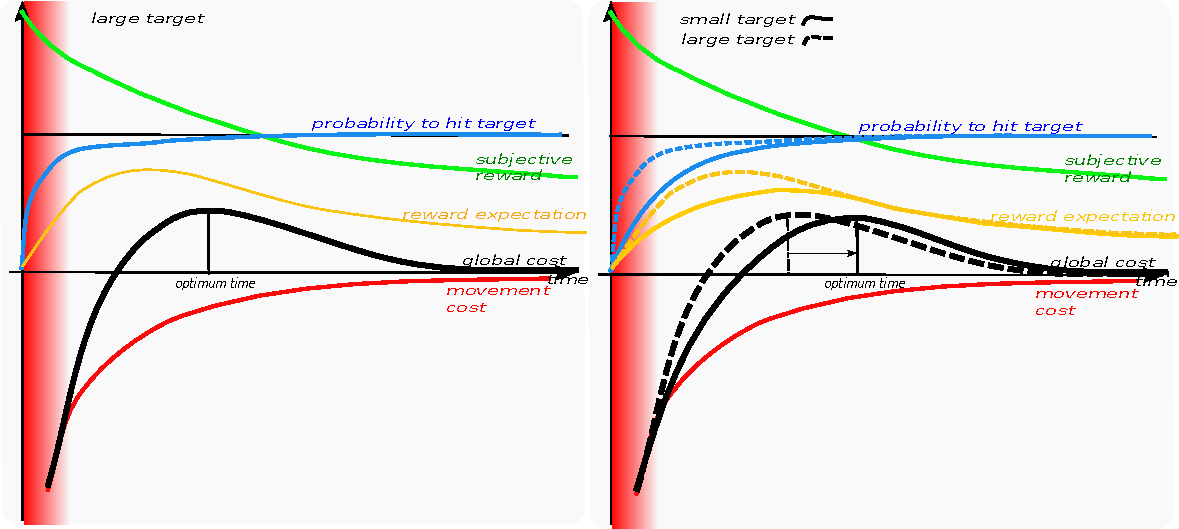
\includegraphics[width=1.0\columnwidth]{images/canu_fig3.pdf}
\caption{Influence of movement time on cost related quantities.
Green: subjective utility of hitting the target; red: muscular energy cost; black: global cost versus reward trade-off. The red area denotes infeasible short times; blue: probability to hit the target; orange:reward expectation (subjective reward times probability).
 A: Sketch of the models in \cite{shadmehr10} and \cite{rigoux12}.
The subjective utility of hitting the reward decreases over time as one is less interested in gains that will occur in a distant future than at the present time. Hitting is less and less costly in terms of efforts as the movement is performed more slowly.
The expected outcome, resulting from the sum of the subjective reward and the (negative) cost reaches a maximum for a certain time. When the outcome is negative (outside the useful interval), one should not move.
B: Sketch of the presented model.
In the case of a larger target, the hitting probability is higher for faster movements (solid lines) than for a smaller target (dashed lines). As a result, the maximum of the reward expectation is shifted towards longer time for smaller targets, and the optimum movement time is also longer for smaller targets.\label{fig:mvt_acc}}
\end{figure}

However, these models do not account directly for basic facts about the relation between movement difficulty and movement duration as captured more than fifty years ago by Fitts' law \cite{fitts54_JEP}.
According to this law, the smaller a target, the slower the reaching movement. 
This is well explained by the so-called {\em speed-accuracy trade-off} (SAT) stating that, the faster a movement, the less accurate it is, hence the higher the probability to miss the target. 
%So a subject reaching too fast may not get the subjective value associated to reaching and should slow down.

In contrast with the models of \cite{shadmehr10} and \cite{rigoux12}, the model of Dean \cite{Dean2007} takes the SAT into account. The key difference with respect to \cite{shadmehr10} and \cite{rigoux12} is that, instead of maximizing a reward, this model maximizes a {\em reward expectation}, i.e. the reward times the probability to get it.

However, the model proposed in \cite{Dean2007} is an abstract model of movement time selection that looks for an optimal trade-off between an externally decayed reward and a SAT that relates the probability of missing to movement time. As such, it does not account for movement execution, neither for the choice of a motor trajectory and its impact on the cost of movement.
The model does not explain Fitts' law, it rather incorporates its consequences into an abstract model of the SAT that is fitted to experimental data.
The mathematical design of the model is based on several simplifying assumptions and it predicts optimal movement times that are systematically shorter than those observed with subjects. The authors of \cite{Dean2007} discuss that this may result from the fact that the model does not take the cost of movement into account.

In this paper, we show that the models of Shadmehr \cite{shadmehr10} and Rigoux \cite{rigoux12} as well as the model of Dean \cite{Dean2007} can be unified into a model that solves the difficulties faced by these previous models. 

This unification is simply implemented by including sensory and motor noise into the optimal control model proposed in \cite{rigoux12}, shifting from a deterministic account of the movement to a stochastic one, in line with the models of \cite{harris98_N,todorov02_NN,todorov04_NN,todorov05_NC,li2006}.

As a matter of fact, in the models of \cite{shadmehr10} and \cite{rigoux12}, the target is given as a single point and the movement is considered as always reaching it, irrespective of the size of the target. In order to fully account for Fitts' law, one must consider the intrinsic dispersion of reaching movements towards a target and the effect of sensory and muscular noise on this dispersion (e.g. \cite{harris98_N}, see \cite{faisal08} for a review), which is not the case of the models of \cite{shadmehr10} and \cite{rigoux12}. 

Considering expectation is a way to account for the fact that, in case of a miss, one would not get the reward, so the global outcome of the movement would only consist of its incurred cost. 

The mathematical way to capture this intuition is presented in Section~\ref{sec:math_model} and illustrated in Fig.~\ref{fig:mvt_acc}(B). Technically, the reward and muscular activation terms in the optimization criterion proposed in \cite{rigoux12} are simply replaced by reward and cost expectation terms. 

With respect to Fig.~\ref{fig:mvt_acc}(A), the new model includes an additional term that expresses the dependency between the size of the target and the probability to hit it, as expressed by the SAT. As can be seen in Fig.~\ref{fig:mvt_acc}(B), if the target is smaller, then the probability to get it is smaller for a given time, thus the reward expectation should itself be smaller. As a result, the optimum time resulting from the optimal combination of this reward expectation with the cost of movement should shift to longer times, which is qualitatively consistent with Fitts' law.

Beyond a theoretical motor control model, this paper proposes a computational model that is tested against a set of experimental phenomena. 

%%%%%%%%%%%%%%%%%%%%%%%%%%%%%%%%%%%%%%%%%%%%%%%%%%%%%%%%%%%%%%%%%%%%%%%%%
\section{Results}
\label{sec:results}

The goal of the computational studies hereafter was to investigate the behavioral properties of the proposed model in order to highlight the differences with respect to \cite{shadmehr10}, \cite{rigoux12} and \cite{Dean2007}.

In a first step we illustrate some basic motor control properties of the model at the level of trajectories and motor cost.
In a second step, we examine the complex relationship between movement time, final dispersion and the expected gain arising from this model.
In a third step, we show that the model globally accounts for Fitts' law.
Finally, we show that it generates an asymmetric velocity profile, where the asymmetry increases with the amplitude of signal-dependent motor noise.

\subsection{Movement cost is not a symmetric function of target location}
\label{sec:perf_xcsf}

In order to investigate basic properties of the motor control model, it is demonstrated on a simulated two-joint planar arm with six muscles taken from the literature and illustrated in Fig.~\ref{fig:arm_model}. This simulated arm model is described in more details in Section~\ref{sec:setup}.

The cost obtained from the different initial configurations described in Section~\ref{sec:apparatus} is shown in Figure~\ref{fig:cost_nops}. 

\begin{figure}[htp]
  \centering
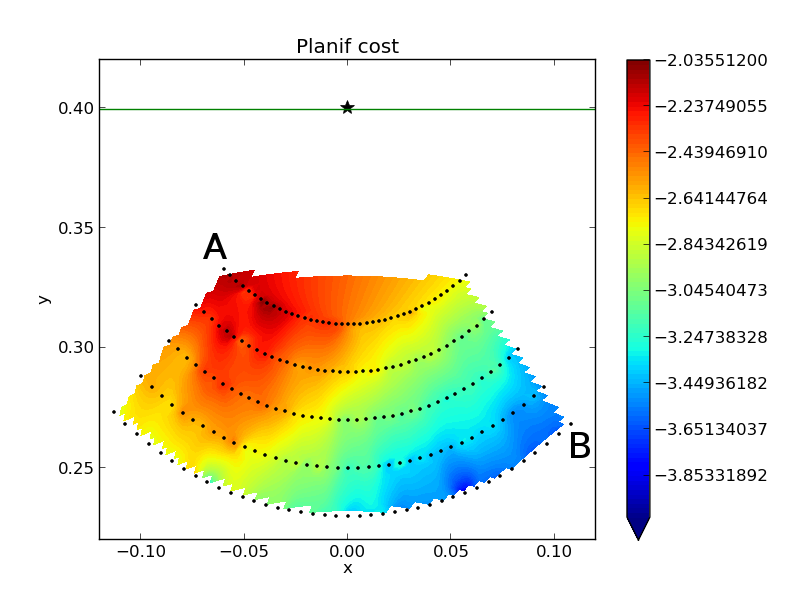
\includegraphics[width=.99\columnwidth]{images/cost_nops}
  \caption{Cost of reaching movements towards the star at $(x=0,y=0.4)$. The movement is stopped when the end-effector crosses the green line at $y=0.4$ (see Methods for details). The color of a point in the reachable space illustrates the cost of a reaching movement from that point. The color-cost correspondence is given by the scale on the right hand-side. As expected, the smaller the distance to the target, the lower the cost. Furthermore, starting from the left hand-side of the goal point results in a lower cost than starting from the right hand-side.
\label{fig:cost_nops}}
\end{figure}

As expected, one can observe that the smaller the distance to the target, the lower the cost. Furthermore, starting from the left hand-side of the goal point results in a lower cost than starting from the right hand-side. This is explained by the fact that the optimal muscular strategy for performing these movements differs depending on the side. Actually, movements starting from the right are performed by moving simultaneously the elbow and the shoulder whereas when starting from the left, only the shoulder is involved, leading to a lower cost.
The muscular activations corresponding to these two situations are shown in Figure~\ref{fig:muscles_LR}. 

\begin{figure}[htp]
  \centering
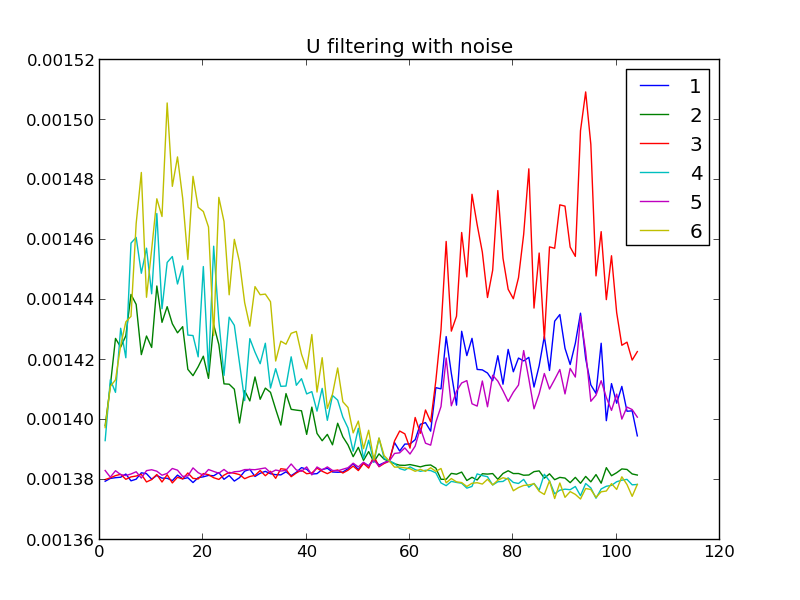
\includegraphics[width=.449\columnwidth]{images/muscles_right2}
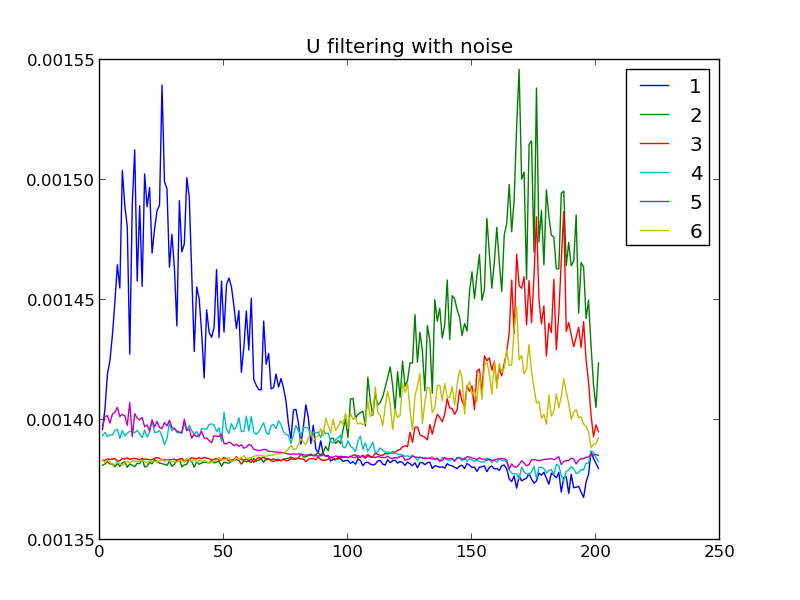
\includegraphics[width=.449\columnwidth]{images/muscles_left1}
  \caption{Muscular activations when performing a reaching movement, either starting from point A in Figure~\ref{fig:cost_nops} (left) or from point B in the same Figure (right).
The numbers in the legend correspond to the muscles numbers in Figure~\ref{fig:arm_model}(b).
One can see that the pattern of activation is very different depending on the initial configuration of the movement, corresponding to two different optimal strategies: when starting from A, only the shoulder is moved, whereas when starting from B, both the elbow and shoulder are moved, resulting in a more complex muscular activation strategy. One can also see that co-contraction is avoided, consistently with the minimum intervention principle.
\label{fig:muscles_LR}}
\end{figure}

One can see that the pattern of activation varies depending on the initial configuration of the movement, corresponding to two different optimal strategies: when starting from a short distance to the left hand-side, only the shoulder is moved, whereas when starting from a long distance to the right hand-side, both the elbow and shoulder are moved, resulting in a more complex muscular activation strategy. One can also see that co-contraction is avoided, consistently with the minimum intervention principle \cite{todorov02_NN}.

\subsection{Relations between movement time, expected gain and final dispersion}
\label{sec:time_perf}

The model presented in this paper is designed to investigate the complex relationships between movement duration, expected gain and final dispersion. In order to perform this investigation, we chose a set of five target sizes ($\{$1mm, 2mm, 6mm, 10mm, 20mm$\}$).
For each target size, we optimized a specific controller (see Methods). For each of these controllers corresponding to each target size, we recorded movement time, final dispersion and performance. The corresponding data is shown in Fig.~\ref{fig:fitts_time}.

\begin{figure}[htp]
  \centering
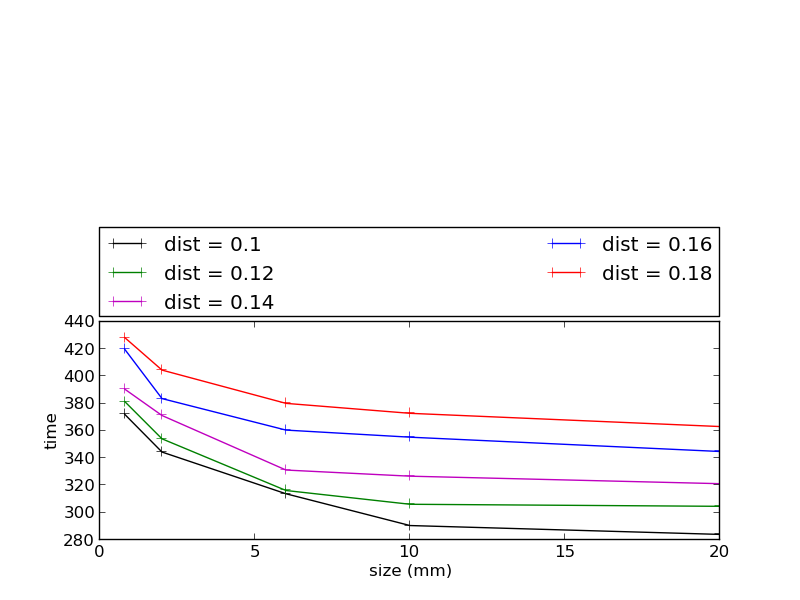
\includegraphics[width=.5\columnwidth]{images/temps_fitts}
%\vspace{-0.5cm}
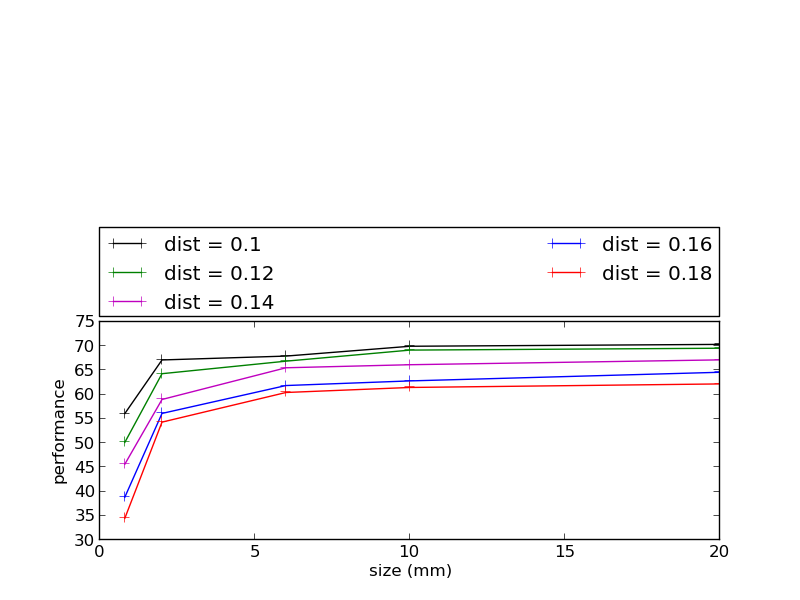
\includegraphics[width=.5\columnwidth]{images/cout_fitts}
%\vspace{-0.5cm}
%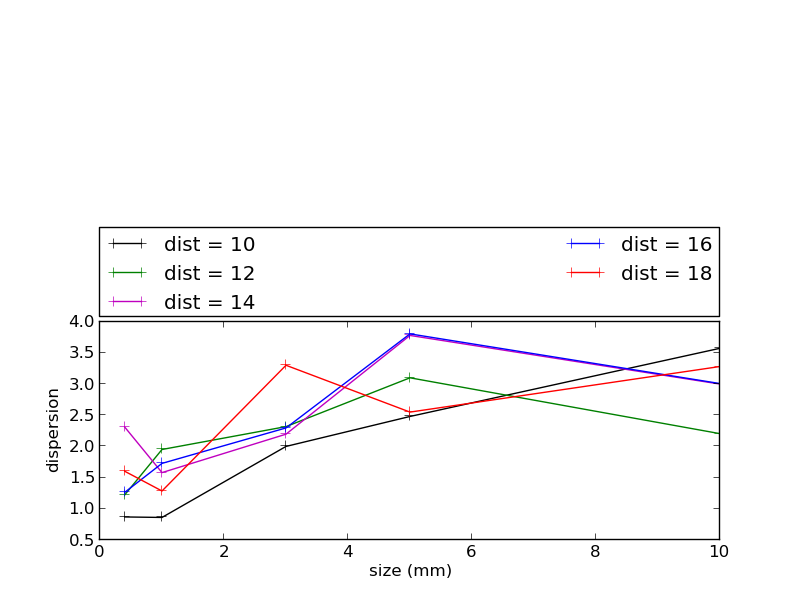
\includegraphics[width=.5\columnwidth]{images/disp_fitts}
  \caption{A: Time of movement for various target sizes and distances. The larger the target, the faster the movement. Additionnally, the further the target, the longer the movement.
B: Expected movement gain for various target sizes and distances. The larger the target, the higher the gain. Additionnally, the further the target, the lower the gain.
%C: Final dispersion for various target sizes and distances.
\label{fig:fitts_time}}
\end{figure}

As illustrated in Fig.~\ref{fig:mvt_acc}(B), the probability to reach the target depends on the size of the target and the time of the movement (or its velocity). More precisely, if the target is smaller, fast movements should fail more often. Thus, as a result of including the accuracy constraint in the model, the optimal movement time resulting from the model described in Fig.~\ref{fig:mvt_acc}(B) should be always longer than the optimal movement time resulting from the model of \cite{rigoux12}.

This is what is observed in Fig.~\ref{fig:fitts_time}(A). One can see that movement time increases when the target is smaller, and also increases with the movement distance, consistently with Fitt's law. 

In Fig.~\ref{fig:fitts_time}(B), one can see that the net expected return is smaller for a larger distance, because the muscular effort for performing a larger movement is larger.

Most importantly, the net expected return increases with the size of the target.
There are two explanations for this fact. First, it means that the benefit in terms of subjective value from reaching the target faster is higher than the increase in cost resulting from a faster movement. Second, if the target is larger, less precision constraints on the movement can result in a better trajectory in terms of muscular activations to reach the target.

%Finally, dispersion increases with the size of the target, but the relationship between dispersion and movement distance is unclear. This last result reveals a limitation of the method, where imperfect optimization and limited sampling due to a large computational cost prevents from obtaining the asymptotic results one would get from a converged optimization.

Finally, Figure~\ref{fig:dispersion} shows an example of the obtained dispersion corresponding to the five targets from a distance of 18cm, using 100 trajectories from the same starting point at $x=0$ to the target.

\begin{figure}[htp]
  \centering
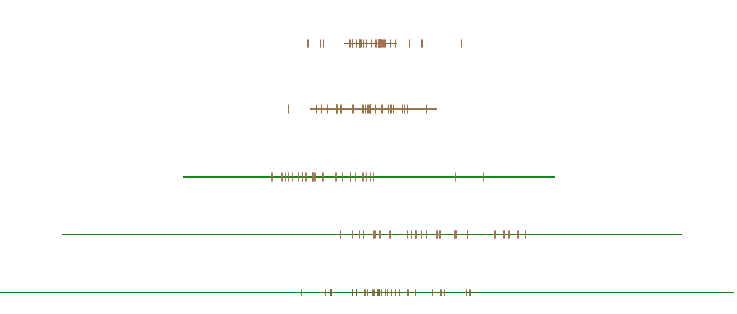
\includegraphics[width=.7\columnwidth]{images/disp_glob}
  \caption{Dispersion resulting from the CEPS controllers optimized for five different target sizes, a movement distance of 18cm and a noise amplitude of 0.4. One can observe that the controller often misses small targets whereas it does not use all the potential dispersion for large targets.
\label{fig:dispersion}}
\end{figure}

One can observe that, when the target is smaller, dispersion is reduced to increase the probability of reaching the target. In order to reduce dispersion, the motion is performed slower, as illustrated in Fig~\ref{fig:fitts_time}. However, for very small targets, the probability to miss the target is not null. This means that, with our parameter settings, it is more optimal to pay the price of a few failed movements than to move slow enough to succeed at all times. There are even target sizes for which reaching may fail whatever the movement velocity.
% This prediction from our model should be checked experimentally with human subjects.

\cite{selen06b} %% comparer les activations musculaires sur une petite cible et une grosse : plus de co-activation?

\subsection{Reproduction of Fitts' law}
\label{sec:fitts}

Fitts' law states that movement time (MT) is linear in its difficulty index (DI), this index being bigger for longer movements and smaller targets. Fitts' law is written:

\begin{equation}
\text{MT} = a + b . \underbrace{\log_2\left(\frac{D}{W}\right)}_\text{DI}
\label{eq:fitts}
\end{equation}

where $D$ is the distance of the movement (denoted with $A$ for amplitude in other papers), $W$ is the width of the target and $a$ and $b$ are linear coefficients. This law was initially studied for one dimensional movements,
and then extended for many other contexts \cite{Soechting1984,Bootsma1994,Laurent1994,Plamondon1997,Smyrnis2000,Bootsma2004}.

From the data presented in Section~\ref{sec:time_perf} and using (\ref{eq:fitts}), we compute $DI$ values for different distances $D$ and target widths $W$. Figure~\ref{fig:fitts} shows the resulting movement time $MT$ over $DI$.

\begin{figure}[htp]
  \centering
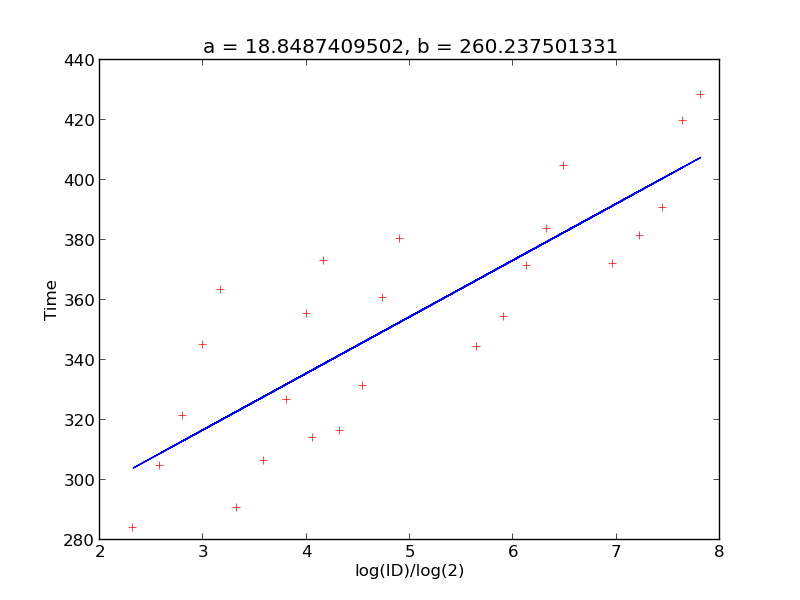
\includegraphics[width=.9\columnwidth]{images/fitts}
  \caption{Reproduction of Fitts law based on the results of Section~\ref{sec:time_perf}.
\label{fig:fitts}}
\end{figure}

One can see that we get a clear linear relationships, thus the data is consistent with Fitt's law.

The obtained values of $a$ and $b$ cannot be compared to empirical data from the human motor control literature given the wide variability of these values accross subjects \cite{crossman1983,mackenzie1989}.

\subsection{Velocity profiles}
\label{sec:velo_prof}

The final dispersion in reaching trajectories is generated by motor noise.
Following the minimum intervention principle from \cite{todorov02_NN}, motor noise being proportional to muscular activation, the only way to decrease motor noise is to decrease muscular activation.

Thus, in order to hit a small target, muscular activations should be small
by the end of the movement, which can result in first instance in less co-contraction and then in less velocity. Furthermore, a slower movement provides a better opportunity for state estimation to compensate for delayed feedback about the position of the end effector. Taken together, those two phenomena contribute to the fact that an optimal controller should generate less velocity by the end of the movement for a smaller target.
So one way to make sure to hit a small target would be to perform a slow reaching movement.

However, as explained above, a slower movement results in a discounted reward,
thus the movement should nevertheless be as fast as possible.

As a consequence, the best option for optimizing reaching accuracy under
temporal constraints consists in being very fast in the beginning of the movement
and much slower in the end. Thus the velocity profile should be asymmetric. The main drive
for this asymmetry being motor noise, the more motor noise, the more asymmetric the movement should be.

This is what we observe in Figure~\ref{fig:velocity}, where velocity profiles are generated
for different amplitudes of motor noise.

\begin{figure}[htp]
  \centering
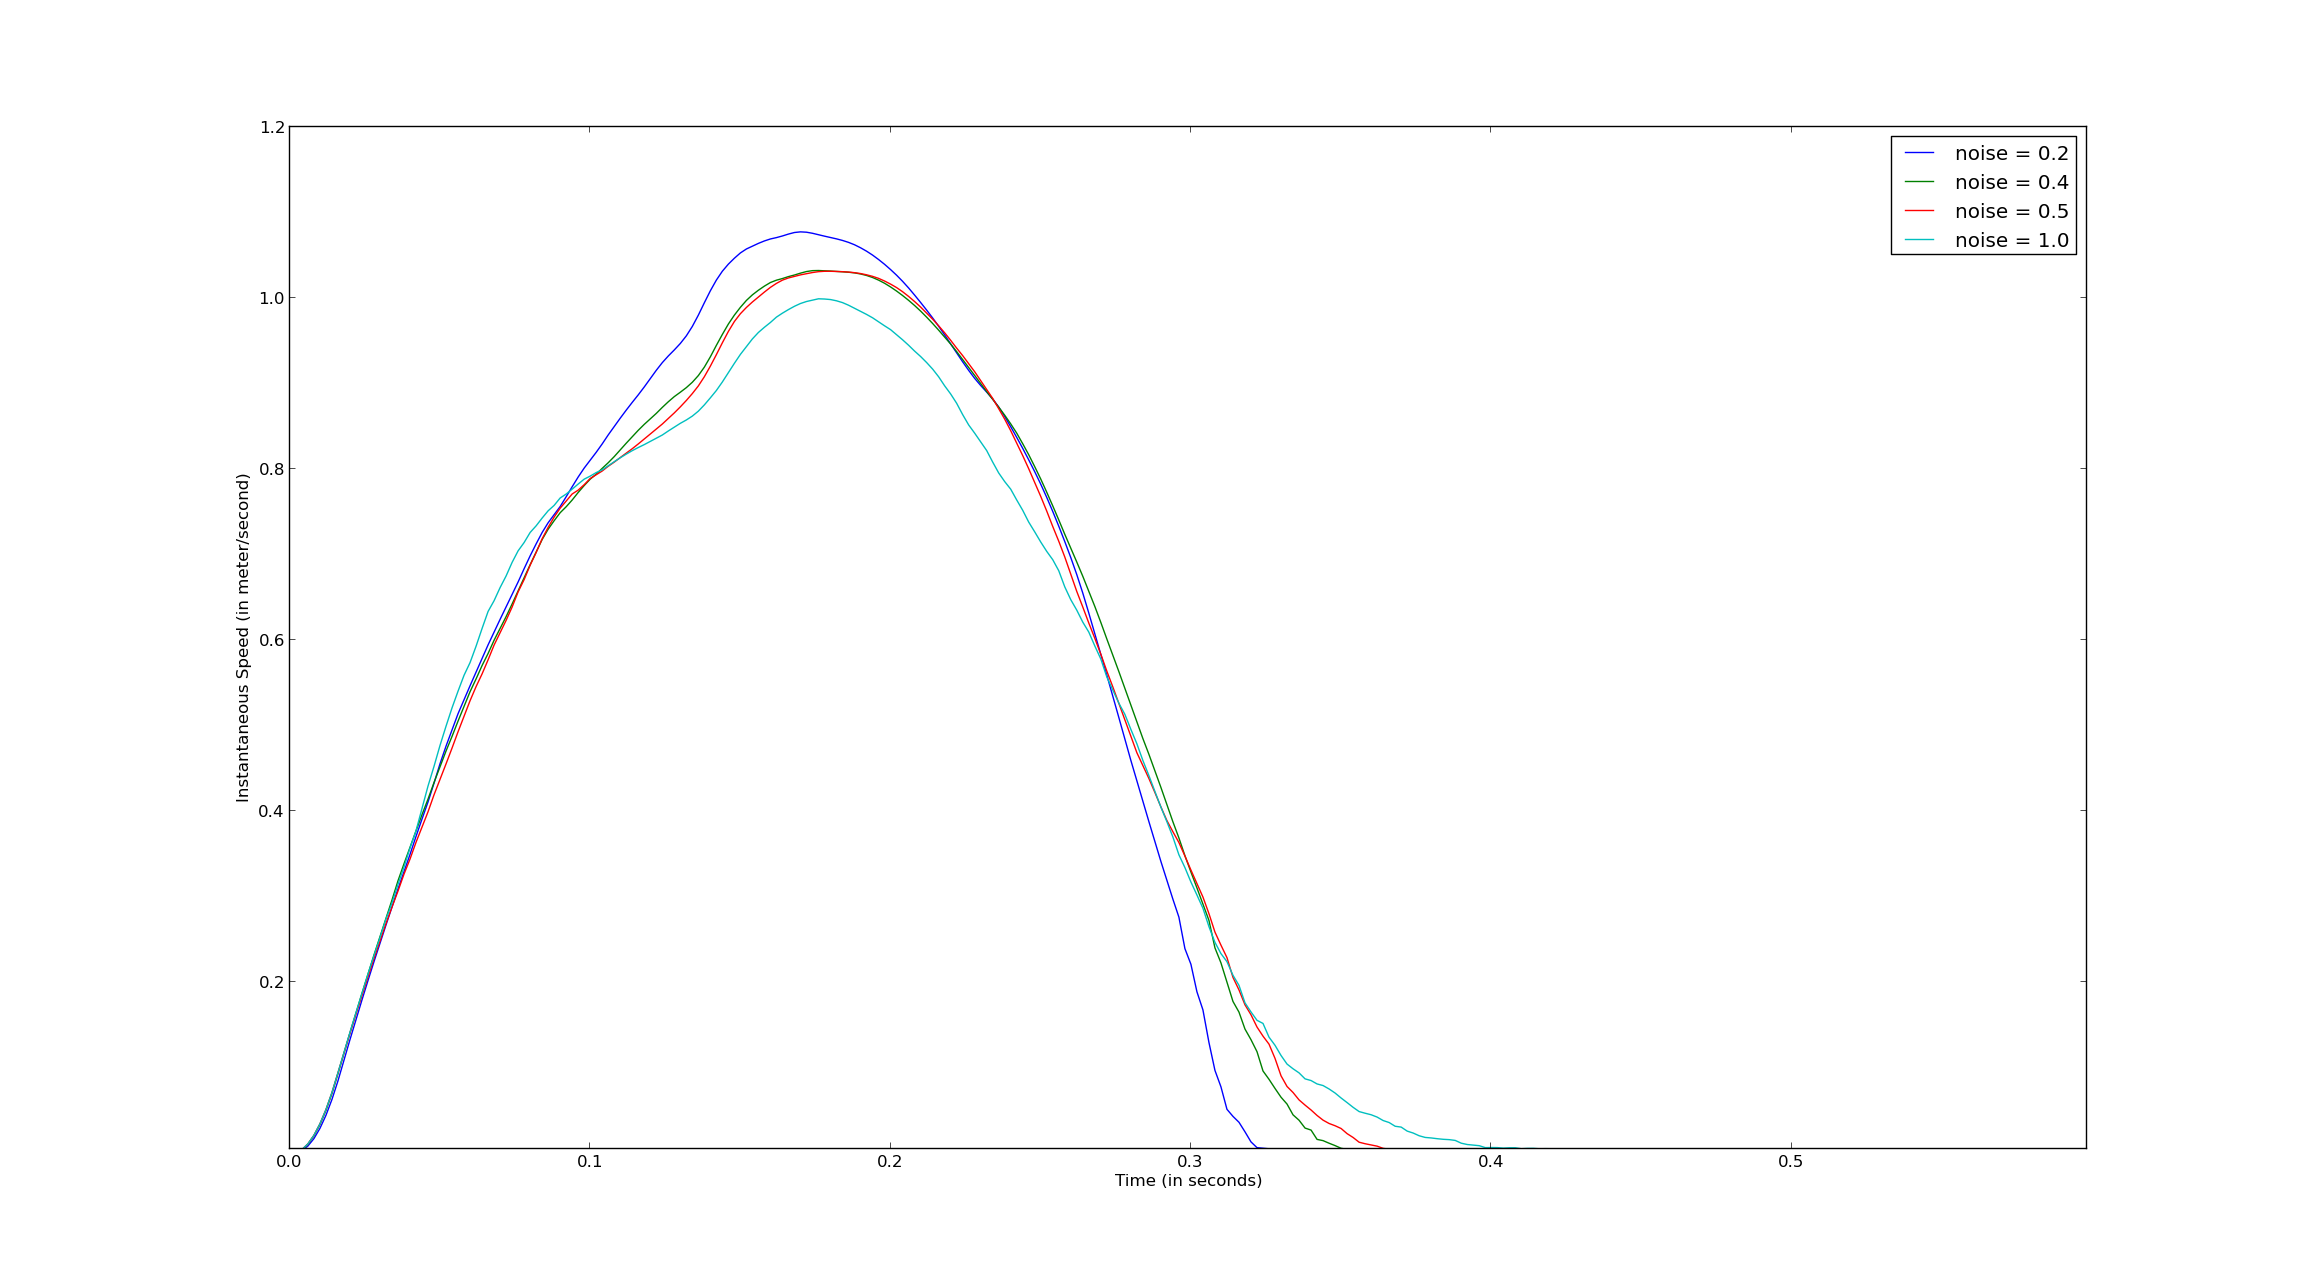
\includegraphics[width=.7\columnwidth]{images/speed_for_diff_noise}
  \caption{Velocity profiles for different amplitudes of noise\label{fig:velocity}.}
\end{figure}

Incidentally, one can observe on the ascending parts of the profiles that we do not get
strictly the shape of a bell curve. This is due to the limited optimization capability
of our methods, given the constraint on the number of samples.

%% \subsection{Adaptation to a moving target}
%% \label{sec:adap_target}

%% One important feature of movement optimization using \ceps is that it can be performed online.
%% As a consequence, \ceps can for instance optimize an \xcsf controller tuned to reach a target at a given position
%% so that the resulting controller generates a distribution of hit points optimized for a
%% target that is placed elsewhere.

%% This property is illustrated in Figure~\ref{fig:moving_target}.

%% {\bf Figure~\ref{fig:moving_target} about here.}

%% \begin{figure}[htp]
%%   \centering
%% 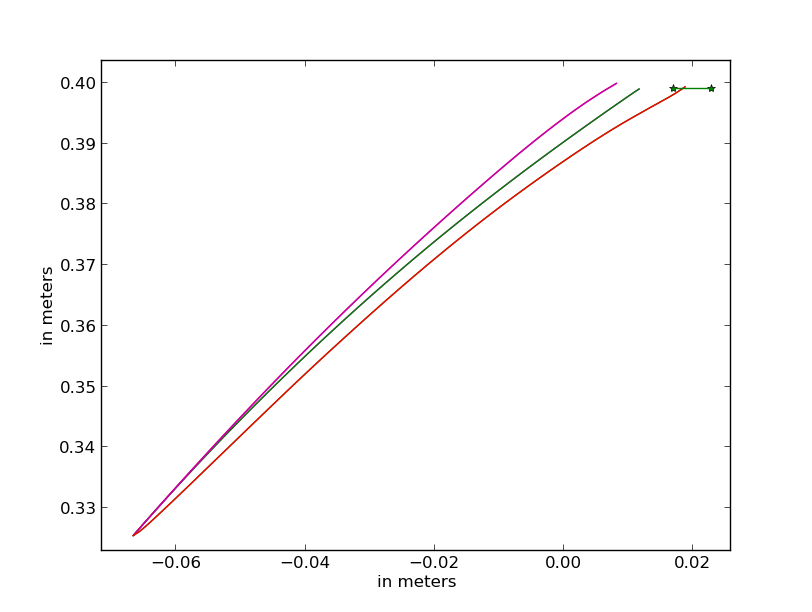
\includegraphics[width=.7\columnwidth]{images/moving_target}
%%   \caption{Mean initial, intermediate and final trajectory when the target is positioned away
%% from the target from which the XCSF controller was trained.\label{fig:moving_target}}
%% \end{figure}

%% One can see that the distribution of hit points is moved towards the new position of the target.
%% This directly results from the tendency of the controller to optimize the reward expectation
%% of the movement.

%% However, if the new position of the target is too far away from the initial one, the
%% probability that the initial movement generation process finds it gets null, and the
%% optimization fails.

%% Actually, if the movement does not get rewarded, the optimal strategy consists in
%% refraining from moving, so as to minimize movement costs. This is also true when the
%% target is so small that the probability to hit it is too small with respect to the
%% expected gain when it is hit.
%% We verified these properties of our model in both contexts (not shown).

%% Those facts arise because our model implements a blind and  local search strategy. In such
%% a context, using some initial training and then a target that is not moved too far
%% from the initial position is a form of {\em reward shaping} that plays an important
%% role in such blind and local search strategy (see e.g. \cite{leblois13}).

%\subsection{Effect of decreasing the reward through time}
%\label{sec:dean2007}

%%%%%%%%%%%%%%%%%%%%%%%%%%%%%%%%%%%%%%%%%%%%%%%%%%%%%%%%%%%%%%%%%%%%%%%%%%%%%%%%%%%%%%%%
\section{Discussion}
\label{sec:discu}


\subsection{Positionning}

When performing a reaching movement towards a target, three inter-related factors must be determined. The first is the potential outcome of a successful or failed movement, characterized by a discounted reward. Movement time is crucial in this factor because more time means a more discounted reward.
The second factor is the cost of the movement, depending on muscular activations and resulting in a velocity profile and a joint-space trajectory. Movement time is crucial in this factor because, for an identical trajectory, shorter time means higher cost. The third factor is the final dispersion, generated by motor noise and imperfectly compensated for by the CNS due to sensory noise and delays. Movement time is crucial in this factor because shorter time means higher dispersion.

The works of \cite{rigoux12} and \cite{shadmehr10} only relate the first two of these factors. By contrast, the model presented in \cite{Dean2007} relates the first and the last factors, without consideration for the second. 

The model presented in this paper addresses the more global inter-relationship between these three factors and provides an optimality criterion that accounts for the strategy of human sujects in this multi-dimensional choice space.

\subsection{Background}

The model presented in this paper is consistent with the stochastic optimal control view of motor control \cite{harris98_N,todorov02_NN,todorov04_NN,todorov05_NC,li2006}. It starts from the fact that, for a small target, the faster the movement, the lesser the chance to hit it {\bf (refs)}.
According to this view, there are two complementary explanations for this fact. First, the motor activation signal descending from the Central Nervous System (CNS) to motoneurons is corrupted with some noise that is proportional to this signal {\bf (refs)}.
Thus a faster movement means more noise, hence more intrinsic dispersion of the final hit point if the arm was controlled in a purely open-loop way.

Second, this intrinsic tendency to dispersion is compensated for by a feedback control loop which is based on state estimation mechanisms.
State estimation itself is based on delayed proprioceptive and perceptive feedback. Thus a faster movement means less time to accurately estimate the state, hence less compensation for dispersion.
As a consequence of both mechanisms, a faster movement results on more final dispersion, hence in a lesser probability to hit a small target.

\subsection{Contributions}

The model proposed here takes the one of \cite{rigoux12} as a starting point. This former model reproduces basic characteristics of motor behavior, as expected from the close relationship with previous optimal control models \cite{gordon94,shadmehr94,todorov02_NN,guigon07a,liu07,guigon08b}. It also explains several phenomena in cost-benefit trade-off tasks \cite{watanabe03,rudebeck06}. The model presented here is equivalent to the one presented in \cite{rigoux12} when the probability to hit the target is set to 1. As a result, it still benefits from the above mentioned properties that are not impacted by this probability.
In this section we show that it solves limitations of the models of \cite{Dean2007} and \cite{rigoux12}.

\subsubsection{The model accounts for target selection bias}

In \cite{Trommershauser2003a}, the authors mention a systematic pointing bias in both the $x$ and $y$ directions for all subjects performing a target hitting experiment. The presence of this bias contrasts with an assumption made in the model of \cite{Dean2007} that, spatial errors being symmetric, the optimal choice of $x$ and $y$ should be in the middle of the circular target.

The proposed model shows that this simplifying assumption does not hold. Indeed, as illustrated in Figures~\ref{fig:cost_nops} and~\ref{fig:muscles_LR}, the optimal strategy to reach a target significantly changes depending on the relative position of the starting point and the target point. As a consequence, when aiming at a large target in the center of the saggital plane in front of himself/herself, an optimal subject would not aim at the center of the target. The optimal aiming point depends on the function relating movement cost to aiming point location, which itself depends on the musculo-skeletal system of the subject. This explains why the bias differs from one subject to the other.

Figures~\ref{fig:cost_nops} and~\ref{fig:muscles_LR} are obtained in a 2D case with a 1D target whereas Dean's experiments were performed in 3D for a circular target. Nevertheless, the asymmetry resulting from the proposed model would also be present in a 3D model. 


\subsubsection{The model directly accounts for Fitts' law}
\label{sec:discu_fitts}
Motor control results are obtained in \cite{rigoux12} in the absence of sensory and motor noise. As such, this model cannot provide a direct account of phenomena relying on the stochasticity of the motor system, such as Fitts' law. Actually, the model of \cite{rigoux12} provides an indirect account of Fitts' law (see \cite{rigoux12}, Fig.~7A). For obtaining these results, the authors have estimated dispersion as a function of velocity considering a constant velocity over the movement, and they have reconstructed the relationship between Difficulty Index and movement time based on the size of a target that would match this estimated dispersion (\cite{rigoux12}, personal communication). So Fig.~7A in \cite{rigoux12} is based on one target size only.

In \cite{Dean2007}, an abstract SAT model is directly fitted to human movement data, without directly calling upond a measured movement dispersion.

In contrast, in Section~\ref{sec:fitts} we have shown that the proposed model accounts for Fitts' law by using several targets and several starting points. In this model, movement velocity is far from constant and dispersion is measured as an effect of motor noise and imperfect state estimation rather than inferred based on an a priori SAT model.

\subsection{Limitations}

\subsubsection{The model does not account for movement planning}
\label{sec:limitations}

In \cite{Trommershauser2003a,Trommershauser2005}, the authors distinguish {\em movement planning} from {\em motor planning}. Movement planning consists in choosing where reaching should aim given a set of rewarded and penalized targets and motor variability. By contrast, motor planning consists in specifying movement execution in advance, in terms of muscular activations at each step of the movement, given a chosen target. Movement planning does not take motor costs into account and does not account for movement time.
Interestingly, the work of \cite{Trommershauser2003a,Trommershauser2005} is focused on movement planning, thus it does not account for the motor trajectory and the choice of movement time as the models of \cite{shadmehr10} and \cite{rigoux12} do.

The model proposed here  might be seen as providing a first stone of the bridge between the work of \cite{Trommershauser2003a,Trommershauser2005} and the one of \cite{shadmehr10} and \cite{rigoux12}.

The model presented in this paper cannot explain the capability to immediately combine information about these interacting targets when they are visible, as reported in \cite{Trommershauser2009}. Some inference mechanism must be assumed to explain this immediate composition capability.
At least part of this inference is probably initiated before movement execution starts.
More generally, there is no mechanism in the model proposed here to account for movement preparation (e.g. \cite{cos11}),
though this stage certainly plays a role in the phenomena studied here.

\subsubsection{Muscular effort or activations?}

It has been shown (ref) that using $||u^2||$ or muscular effort or... results in very similar movements.

\subsubsection{Exponential versus hyperbolic discounting}

The proposed model starting from the one in \cite{rigoux12}, it inherits from this model an exponential discounting of the reward through time. In an alternative model, \cite{shadmehr10} rather suggests
an hyperbolic discounting approach, in line with many other authors (e.g. \cite{prevost10}).
At this stage, we consider that the debate between diverse discounting approaches is far from
close (see e.g. \cite{green96}) and using a different discounting approach would not
fundamentally change the results presented in this paper.

\subsubsection{Expectation over reward or expected gain}

The proposed model computes the expectation over the reward part rather than on the sum of the reward and the movement cost. The intuition behind this choice is that the reward term varies a lot depending on whether the target was hit or not whereas the movement cost is grossly constant over movements from the same point to a same target. If the movement cost was actually constant over movements, it could be left out of the expectation term without harm. To discriminate between both potential models, one should investigate experimental settings where the cost of movements varies a lot, for instance using force fields. This is left for future work.

\subsubsection{Imperfect optimization}

Results in Figures~\ref{fig:fitts_time}(C) and~\ref{fig:velocity} show that the incremental optimization process used in this paper (see Section~\ref{sec:methods}) was not given enough iterations to reach a global optimum.

%% Dans le cas de \ref{fig:fitts_time}(C), c'est peut-être juste un problème de sampling sur les dispersions => voir si on peut améliorer...

\subsection{Predictions}

The computational study presented in this paper can be seen as generating a number of predictions that remain to be tested experimentally.

First, in the context of planar reaching movements towards a large target in front of the subject, we predict a tendency to move the distribution of hit points to the left, because movements towards the left are less expensive than movements along the saggital plane.

Second, the model proposed here progressively optimizes its distribution of hit points based on the gain resulting from previous hits.
Actually, the model proposed here addresses a situation that is quite different from the one experimented in the work of Trommersh\"{a}user et al. \cite{Trommershauser2003a,Trommershauser2003b,Trommershauser2005}.
Their work considers a situation where the subject can see the target and decides where to aim based on this available information. Decision is described as an inference process based on global information. In our model, by contrast, the search for the right hit point dispersion is a local trial-and-error process. Pre-training orients the controller towards an initial distribution of hit points, then the optimization process adapts this controller to a specific target but the controller is not given any prior information about the size or location of this target. It is only informed whether the target was hit or not through the reward feedback.

Thus, experimentally, the model presented in this paper would correspond to a situation where a subject is vaguely informed about the location of the target but has to adapt its reaching movement to maximise the outcome through trial-and-error. To our knowledge, this situation has never been studied experimentally in the litterature.

The most closely related situation is the one described in \cite{Battaglia2007}, 
where the target is progressively shown to the subject by plotting more
and more random points drawn according to the spatial distribution of the reward. Thus, in a way,
the subject discovers the target through time, rather than through trial-and-error.

In the situation corresponding to the proposed model, it would be interesting to determine
experimentally the circumstances
under which a subject sacrifices accuracy depending on the target location, its size,
its rewarding value and timing constraints over the movement. All the corresponding
data could be checked against the predictions of the proposed model.
In particular, one can anticipate that, if the reward gets null after a short time, subjects
should perform the movement very fast at the expense of accuracy, given that hitting a rewarded target only
part of the time is still better that receiving no reward at all over all trials.

%% \subsection{Conclusion and future work}
%% \label{sec:conclu}

%% In this paper, we have proposed a mathematical model that accounts for the time of a reaching movement taking the expected gain and accuracy constraints into account.

%% When compared at the mathematical formalization level, the main departure of this model from \cite{rigoux12}
%% comes from the fact that it optimizes a distribution of goal point so as to match a target of a given size, instead of aiming at a single point in an infinitely large target.
%% We have shown that, with this property, our model can account both for a speed-accuracy trade-off characterized by Fitts' law and for the emergence of a movement time that results from a cost-benefit trade-off.

%% Beyond testing its predictions experimentally,
%% the work presented in this paper opens several directions for future work. 

%% First, the model should be extended to overcome the limitations pointed in Section~\ref{sec:limitations} in terms of both computational methods and explanatory power. In particular, the model could be checked against the experimental data of \cite{Dean2007}, provided some way to model the effect of the reward devaluation on the subjective discount of this reward, as expressed in (\ref{eq:expectation}). 
%% Furthermore, the model may also account for the results
%% of \cite{Hudson2008}, where the subject is rewarded only if the target is hit during a given time window.

 
%% Under this perspective, our method is just another optimization method that provides nearly
%% optimal results faster than the one described in \cite{rigoux12}.
%% As a result of this perspective, our model generates a set of predictions about
%% the properties of optimal or close to optimal movements.

%% Another fruitful perspective would consist in considering the proposed methods as accounting for an
%% online, local search process that optimizes reaching accuracy through a trial-and-error
%% process. This perspective is endowed with a potentially richer explanatory power, but more remains
%% to be done to expand the scope of the model in this direction.
%% Under this online optimization perspective, an agmented version of the model presented here
%% could also be used to account for the work of \cite{izawa08} and \cite{diedrichsen10}.

\subsection{From motor control to motor learning}

The perspective taken here about our model consisted in considering the proposed
methods as a tool to get optimal behaviours with respect to the cost function
defined by Eq.~(\ref{eq:expectation}).

By the way, this method optimizes a parametric controller for a given target size and location by trial-and-error, without knowing these size and location in advance. For a particular context, it empirically optimizes the trade-off between cost and accuracy by tuning the motor input so that velocity generates the optimal dispersion for the given target.
In that respect, the model might be considered under a motor learning perspective
that would try to explain how we may learn optimal reaching movements from trial-and-error,
but this is beyond the scope of this paper.

\section{Material and methods}
\label{sec:methods}

In the first part of this section, we describe the theoretical background of the model.
In a second part, we describe how we obtain a computational model that optimizes
the cost function described in (\ref{eq:expectation}) for different contexts.
Finally, the simulated arm and experimental apparatus used to model reaching
are described in Section~\ref{sec:setup}.

\subsection{Mathematical formulation of the model}
\label{sec:math_model}

The cost function $J(\vec{u})$ proposed for a control $\vec{u}$ in the model of \cite{rigoux12} is

\begin{equation}
\label{eq:criterion}
 J(\vec{u}) = \int_0^{\infty} e^{-t/\gamma} [ \rho R(\vec{s}_t) - \nu L(\vec{u}_t) ] dt
\end{equation}

where $R(\vec{s}_t)$ is the immediate reward function that equals $1$ at the goal point (also called rewarded state) and is null everywhere else. The function $L(\vec{u}_t)$ is the movement cost. The authors of \cite{rigoux12} take $L(\vec{u}_t) = \|\vec{u}_t\|^2$, as in many motor control models. 
The continuous-time discount factor $\gamma$ accounts for the ``greediness'' of the controller, i.e. the smaller $\gamma$, the more the agent is focused on short term rewards.
Finally, $\rho$ is the weight of the reward term and $\nu$ the weight of the effort term.
In all experiments presented here, based, on the previous work from \cite{rigoux12}, we took $\gamma=0.998$, $\rho=1$ and $\nu=3000$.

A near optimal deterministic policy to solve this problem is obtained through a computationally expensive variation calculus method (see \cite{rigoux_these} for details).
Given that the policy does not take the presence of noise in the model of the plant into account, 
the actions must be computed again at each time step depending on the new state reached by the plant
which further contributes to the cost of the method.
The controller resulting from this model is called the \ops (for Near-Optimal Planning System) in the rest of this paper.

Now let us consider the integration of accuracy constraints. Instead of a deterministic controller, the new model is based on a stochastic controller where the rewarded state is reached or not. As a result, the outcome of a large set of movements performed with noise is computed as the value of the reward mutiplied by the probability to obtain it over the different movements. 
Mathematically, the value multiplied by the probability is called the expectation.

Taking the probability to reach the target into account as described above, the new optimization criterion is written

\begin{equation}
\label{eq:expectation}
 J(\vec{u}) = \int_0^{\infty} e^{-t/\gamma} \E[ \rho R(\vec{s}_t) - \nu L(\vec{u}_t) ] dt
\end{equation}

where $\E[]$ stands for the expectation of the cumulated reward, and $R(\vec{s}_t)$  equals $1$ if the end effector hits the target.

\subsection{Incremental stochastic optimization}
\label{sec:xcsf_ceps}

The optimal control problem arising from a cost function including a reward expectation cannot be solved analytically. The reward expectation itself must be estimated empirically through a set of attempts to hit the target (these attempts are called ``\rols'' hereafter). The more \rols, the better the estimate of the reward expectation. In \cite{rigoux12}, the simpler optimal control problem was solved with a numerical variation calculus method called the ``Near-Optimal Planning System'' (\ops) hereafter. This method is computationnally expensive, it takes about 10 minutes for generating one reaching trajectory on a standard computer. As a consequence, it cannot be used as such to empirically determine the reward expectation for a given problem configuration.

To circumvent this difficulty, the computational model presented in this paper relies on a two-step approach. First, we approximate the \ops using a nonlinear function approximation technique named \xcsf.\xcsf is a regression algorithm that can approximate a function in a large continuous space \cite{wilson2001,wilson2002}. It generates a parametric model of the approximated function as a Gaussian mixture of linear models, i.e. a collection of local linear models bound to Gaussian support functions. A more complete description of \xcsf can be found in \cite{butz2004,butz2008,sigaud11_ras}. The result is a parametric controller that approximates the function relating the state $\vec{s}$ of the system to the adequate control input $\vec{u}$ the \ops would provide in that state.
This approximated function is called the \xcsf controller. It is trained by using trajectories generated by the \ops as input samples, using  the cost function described in (\ref{eq:criterion}). Its parameters are the weights of all local linear models learned with \xcsf.

As described in \cite{marin11_gecco}, this controller mimics the \ops in the limited region where it has been trained, but it reacts several orders of magnitude faster because the result of the optimisation process is ``compiled'' into the controller parameters. From this much faster controller, it becomes possible to empirically estimate a discounted reward expectation from many \rols.

In a second step, the \xcsf controller is re-optimized with respect to the cost function (\ref{eq:expectation}) for different target sizes and different sets of initial positions. This optimization is performed using a variant of the Cross-Entropy Method (\cem) \cite{Rubinstein97} illustrated in Fig.~\ref{fig:cross-entropy}. 

\begin{figure}[hbt]
\centering
	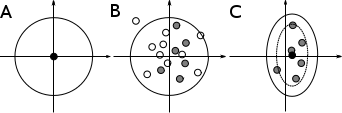
\includegraphics[width=0.6\columnwidth]{images/cross-entropy_simple}
	\caption{Schematic view of the Cross-Entropy method.
A: Start with the normal distribution $\Nu(\mu,\sigma^2)$.
B: Draw sample parameters from this distribution, evaluate them and select the best ones (in grey).
C: Compute the new $\mu$ and $\sigma^2$ (adding some noise) and go to A.
	\label{fig:cross-entropy}}
\end{figure}

Given the initial \xcsf controller learned from \ops demonstrations, the method consists in optimizing the parameters of this controller by a local stochastic search method. New \rols are performed with varying parameters for all local linear models around those of the current controllers, and the parameters that give rise to a better performance with respect to the cost function (\ref{eq:expectation}) are retained in the new current controller. For more details about the methods, see \cite{marin11_gecco}.

We use the JavaXCSF \cite{Stalph2009} implementation of \xcsf, and the main code for the experiments as well as the \ceps algorithm are also implemented in Java.
The experiments are run on a Intel Core 2 Duo E8400 @ 3 GHz with 4 GB RAM.

\xcsf is tuned as follows. The maximum number of local linear models (population) is set to $200$. Learning is stopped after $200,000$ iterations. The input are normalized: the target and current positions are bounded by the reachable space and the speed is bounded by $[-100, +100]~rad.s^{-1}$. The default action $\vec{u}_{default}$ is set to a vector of zeros i.e., no muscular activation. After tuning empirically the parameters, the learning rate \texttt{beta} is set to $0.1$, the accuracy factor \texttt{alpha} is set to $1.0$ and the deletion threshold \texttt{delta} is set to $0.1$. Compaction, randomization and multithreading are disabled to improve reproducibility of the results \cite{Stalph2009}.

%%%%%%%%%%%%%%%%%%%%%%%%%%%%%%%%%%%%%%%%%%%%%%%%%%%%%%%%%%%%%%%%%%%%%%%%%%%%%
\subsection{Arm model and experimental apparatus}
\label{sec:setup}

There are several models in the literature that combine a simple two joint planar rigid-body dynamics model with a muscular actuation model. Most of these models \cite{katayama93,mitrovic08_SAB,li2006} are defined in the sagittal plane and
ignore gravity effects, an exception beingd \cite{Kambara2009} that lies in the vertical plane and takes the gravity force into account.

Apart from this exception, the differences between the models above mostly lie in the muscular actuation component.

Our model is also a two joints planar arm in the saggital controlled by 6 muscles, illustrated in Fig.~\ref{fig:arm_model}, where the muscular actuation model is taken from \cite{katayama93} (pp.~356-357) as cited by \cite{mitrovic08_SAB}.

\begin{figure}[hbt]
\centering
	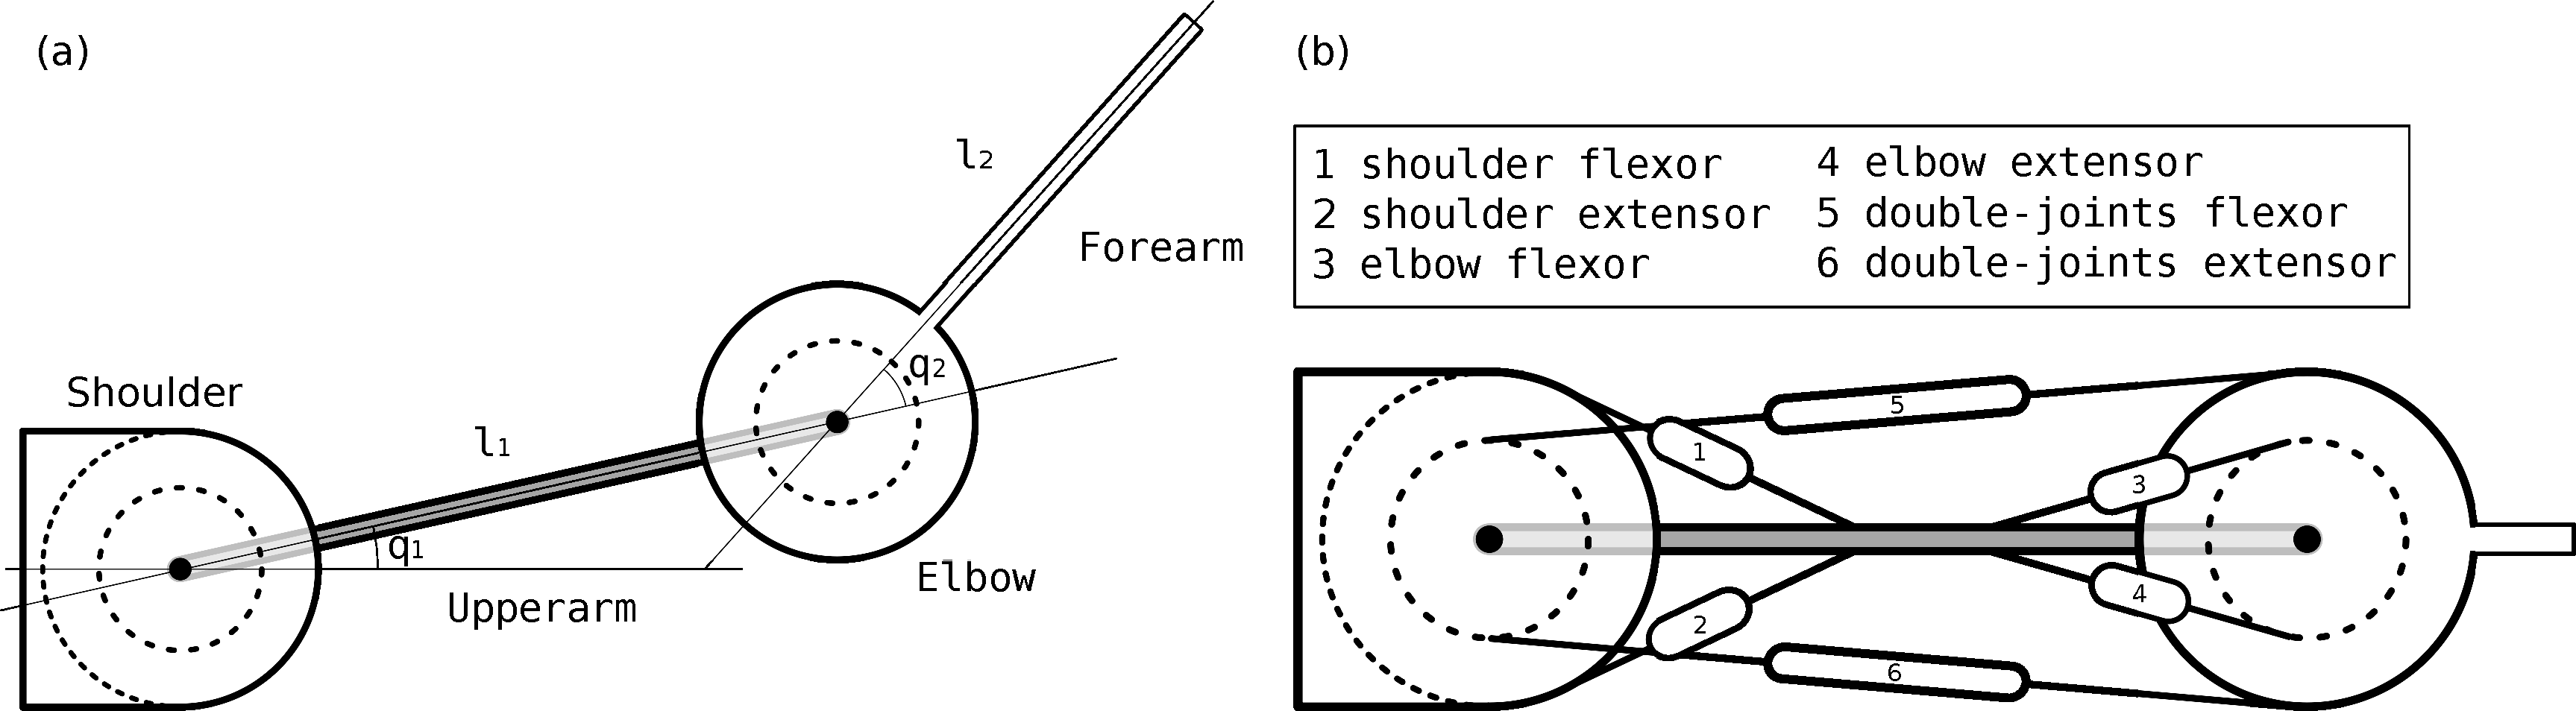
\includegraphics[width=0.9\columnwidth]{images/arm_model_horiz}
	\caption{Arm model. (a) Schematic view of the arm mechanics. (b) Schematic view of the muscular actuation of the arm, where each number represents a muscle whose name is in the box.}
	\label{fig:arm_model}
\end{figure}

Figure~\ref{fig:arm_model} shows the arm with the positionning of the muscles.
Table~\ref{arm_model_params} in Appendix~\ref{sec:nomen} reminds the nomenclature of all the parameters and variables of the model. 

\subsubsection{Rigid-body dynamics}
\label{sec:arm_dynamics}

The rigid-body dynamics equation of a mechanical system is:

\begin{equation}
\label{eq:rbd}
    \ddq = \ms{M}(\q)^{-1} (\vt - \ms{C}(\q, \dq) \dq - \vs{g}(\q)  - \ms{B} \dq) 
\end{equation}

where $\vs{q}$ is the current articular position, $\dq$ the current articular speed, $\ddq$ the current articular acceleration, $\mat{M}$ the inertia matrix, $\vs{C}$ the Coriolis force vector, $\vs{\tau}$ the segments torque, $\vs{g}$ the gravity force vector and $\vs{B}$ a damping term that contains all unmodelled effects.

Here, $\vs{g}$ is ignored since the arm is working in the sagittal plane.

All angles are expressed in radians.

Given the arm parameters $m_1 = 1.4, ~ m_2 = 1.1, ~ l_1 = .30, ~ l_2 = .35$,
$s_1 = .11, ~ s_2 = .16, ~ d_1 = .025, ~ d_2 = .045$, where $m_i$ is the mass of segment $i$, $l_i$ the length of segment $i$, $s_i$ the inertia of segment $i$ and $d_i$ the distance from the center of segment $i$ to its center of mass, the inertia matrix can be computed as
$
 \mat{M} = \begin{bmatrix}
           k_1 + 2 k_2 \cos(q_2)   &  k_3 + k_2 \cos(q_2) \\%[0.3em]
           k_3 + k_2 \cos(q_2)     &  k_3
          \end{bmatrix}
$, with $k_1 = d_1 + d_2 + m_2 l_1^2, ~ k_2 = m_2 l_1 s_2, ~ k_3 = d_2$.

The Coriolis force vector is given by
$
\vs{C} = \begin{bmatrix}
           -\dq_2 (2 \dq_1 + \dq_2) k_2 \sin(q_2) & \dq_1^2 k_2 \sin(q_2)
          \end{bmatrix}.
$

The damping term is 
$\vs{B} = \begin{bmatrix}
           .05 & .025 \\
          .025 & .05
     \end{bmatrix} \dq.$\\

The computation of the torque $\tau$ exerted on the system given an input muscular actuation $\vs{u}$ is explained in the next section.

\subsubsection{Muscular actuation}

Our muscular actuation model is taken from \cite{katayama93}. It is a simplified version of the one described in \cite{li2006} in the sense that it uses a constant moment arm matrix $\mat{A}$ whereas \cite{li2006} is computing this matrix as a function of the state of the arm.

From \cite{katayama93}, we take the maximum force exerted by each muscle as

\begin{align*}
  \vs{f_{\max}}   & = \begin{bmatrix}f_{\max1} & f_{\max2} & f_{\max3} & f_{\max4} & f_{\max5} & f_{\max6}\end{bmatrix} \\
                  & = \begin{bmatrix}700 & 382 & 572 & 445 & 159 & 318\end{bmatrix}^\top \\
\end{align*}

and the moment arm matrix is

\begin{align*}
  \ms{A}          & = \begin{bmatrix}
    A_{11} & A_{21} & A_{31} & A_{41} & A_{51} & A_{61} \\
    A_{12} & A_{22} & A_{32} & A_{42} & A_{52} & A_{62} \\
  \end{bmatrix}^\top \\
  & = \begin{bmatrix}
    .04 & -.04 &    0 &     0 & .028 & -.035 \\
    0 &    0 & .025 & -.025 & .028 & -0.35 \\
  \end{bmatrix}^\top.\\
\end{align*}

Finally, given an action $\vs{u}$ corresponding to a raw muscular activation as output of the
controller, the muscular activation
is augmented with Gaussian noise using $\vs{\tilde{u}} = \log(\exp(\kappa \times \vs{u}_t \times (1+\mathcal{N}(0,\mat{I}\sigma_u^2))) + 1) / \kappa$, where $\times$ refers to the element-wise multiplication, $\mat{I}$ is a $6 \times 6$ identity matrix.
and $\kappa = 25$ is the Heaviside filter parameter, and the input torque 
is computed as $\vs{\tau} = \mat{A}^\top (\vs{f_{\max}} \times \vs{\tilde{u}})$.

Given (\ref{eq:rbd}), the simulator uses the Euler method to compute the evolution of the system, with a time step of $\Delta t = 2$ ms.

\subsubsection{Motor noise and state estimation}

In order to reproduce Fitts' law and to study the structure of movement variability, taking sensory and motor noise into account is necessary. 
In order to get an adequate dispersion, we considered multiplicative motor noise $w_t$ with $p(w) \sim \mathcal{N}(0, 0.4)$ and additive sensory noise $\nu_t$ with $p(\nu) \sim \mathcal{N}(0, 0.0004)$. The feedback delay is $100$ms.
State estimation was performed with an extended Kalman filter as described in \cite{guigon08a}. 

\subsubsection{Experimental apparatus}
\label{sec:apparatus}

In most experiments where a subject has to reach a target, either in monkeys (e.g. \cite{kitazawa98}) or humans \cite{Trommershauser2003a,Dean2007,Battaglia2007,Hudson2008,Trommershauser2009}, the target is displayed on a vertical screen and the subject performs a trajectory in the sagittal plane that the screen intercepts.
Our experimental apparatus reproduces such a scene in the sagittal plane.

Figure~\ref{fig:arm_workspace} shows the experimental apparatus for reaching.
Cartesian coordinates (in meters) are expressed with 
respect to the position of the shoulder, taken as origin $(x=0, y=0)$.
The arm is shown together with the screen and the set of starting positions of the tested movements. In all experiments the target is located at the same place, but its size changes. The starting configuration is varied systematically over all movements so as to investigate the effect of the distance travelled through the movement.

\begin{figure}[t]
\centering
	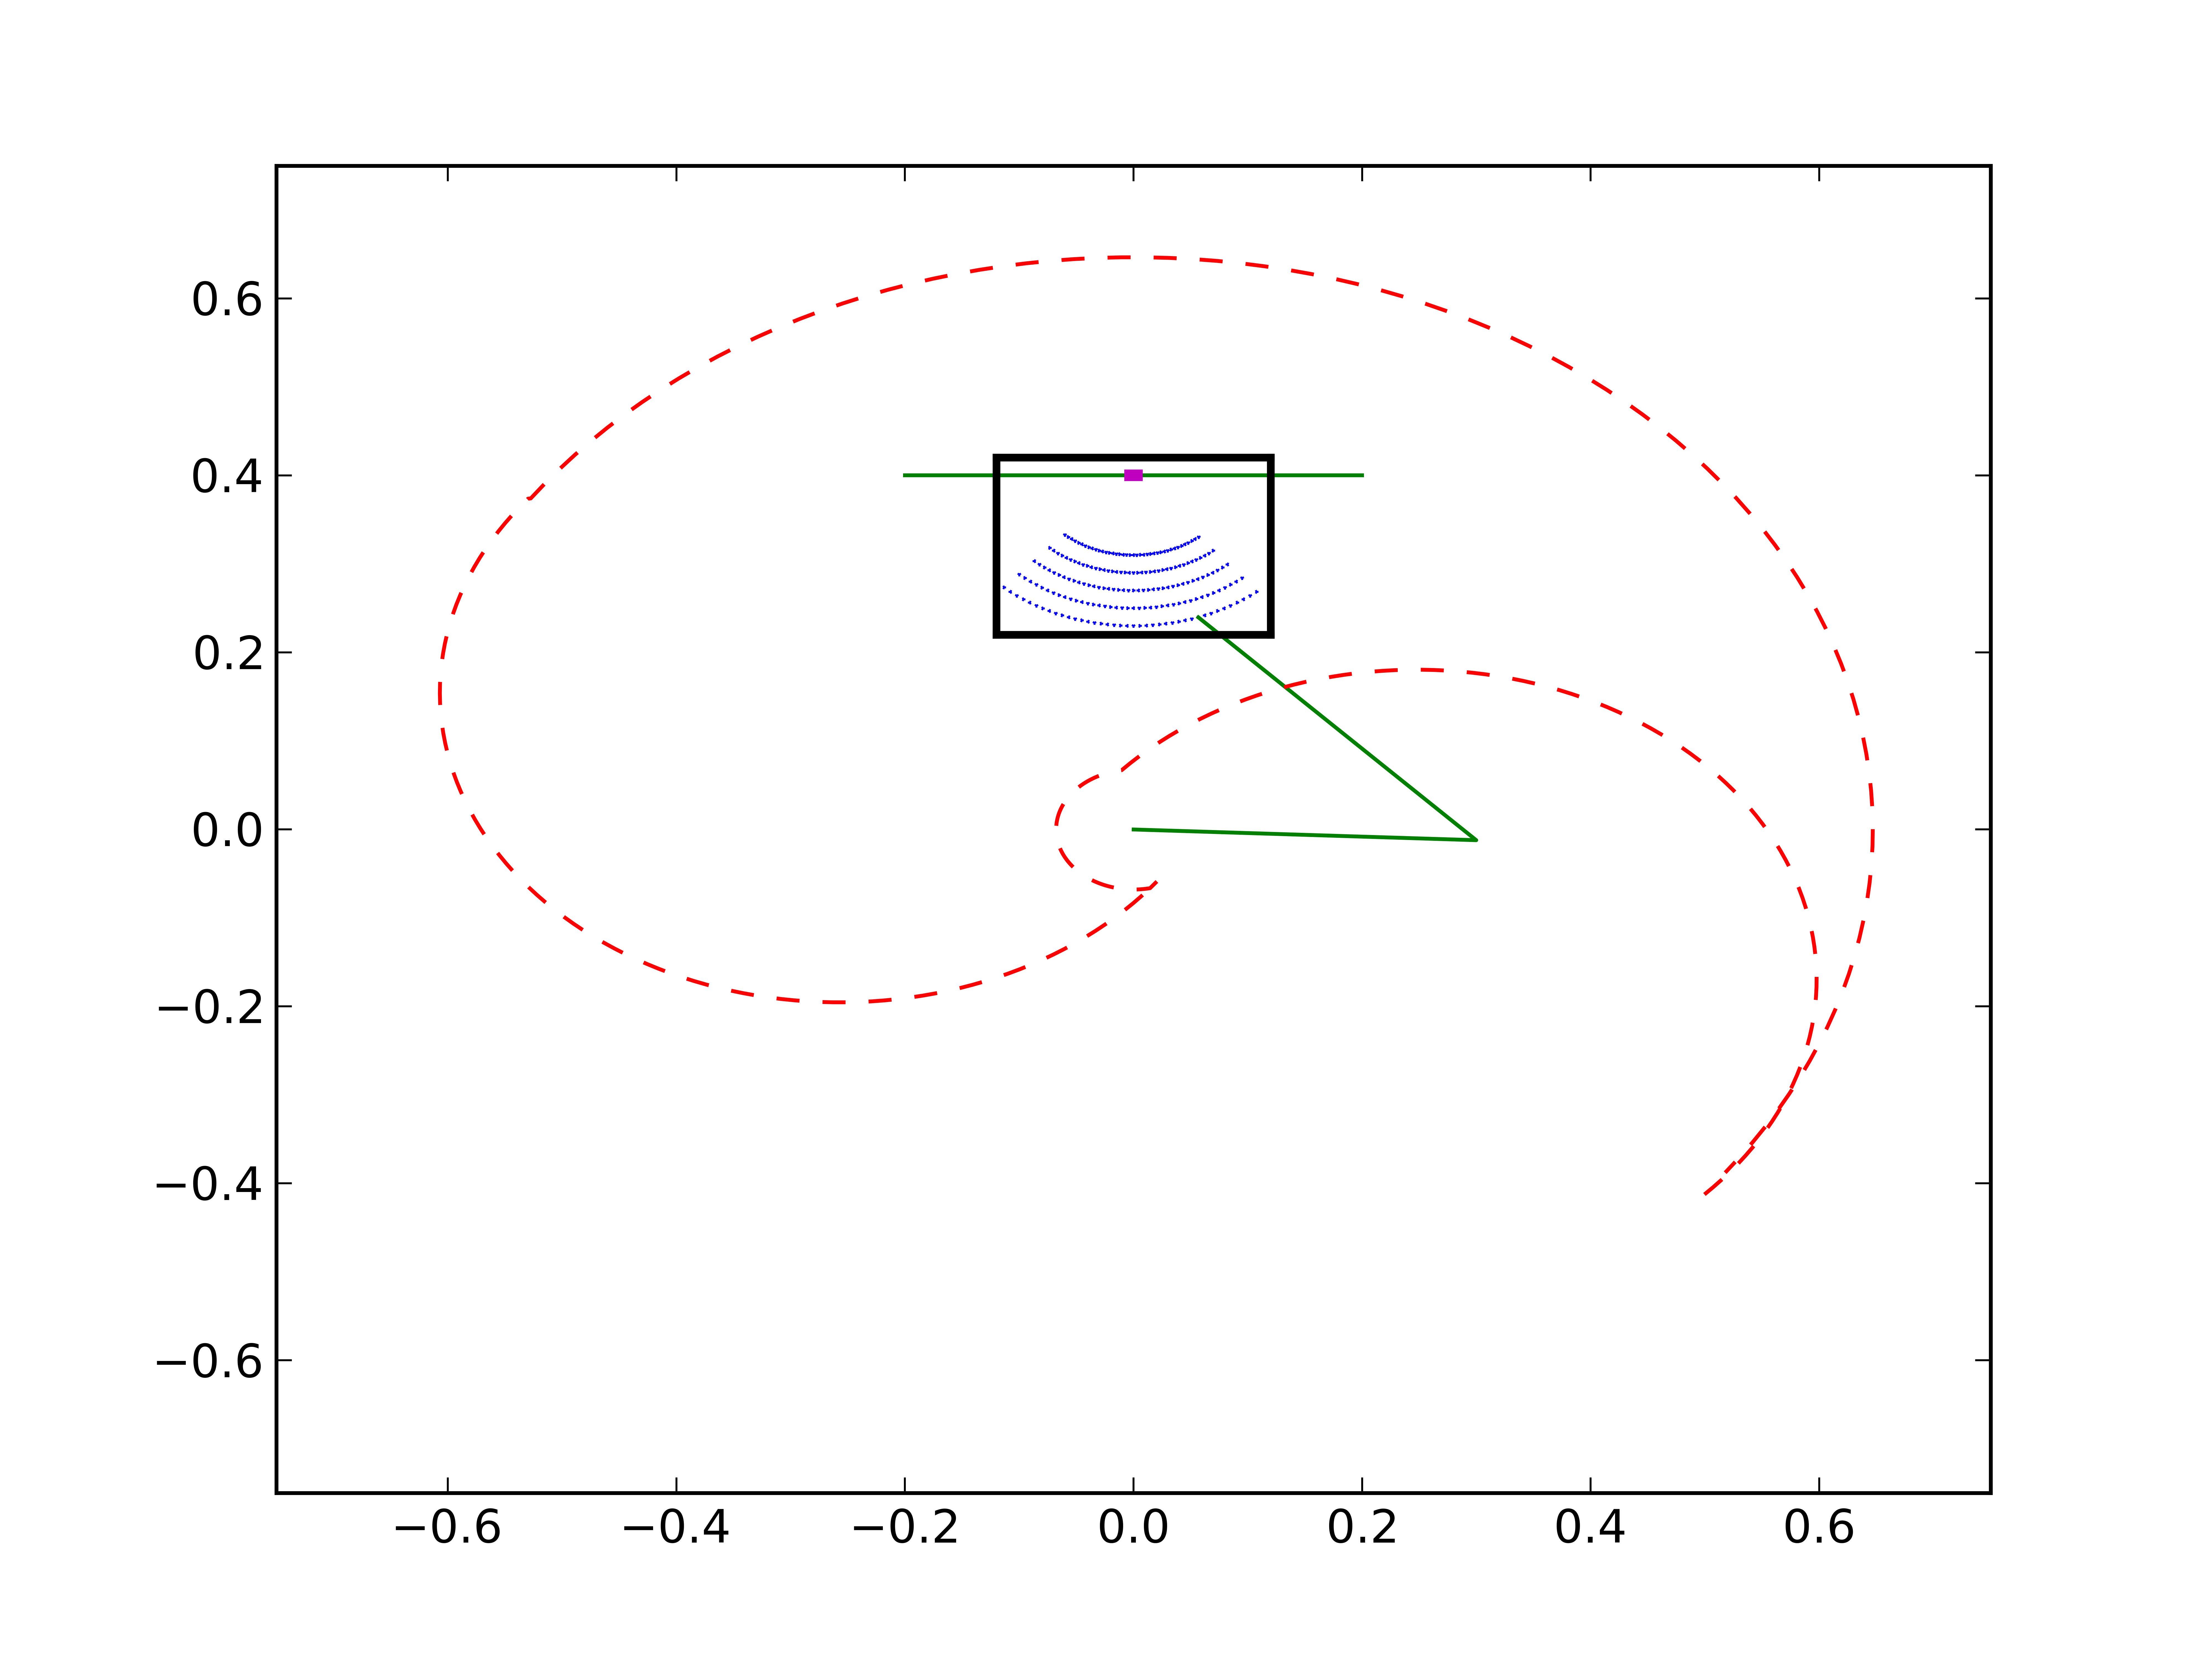
\includegraphics[width=0.8\columnwidth]{images/workspace}
	\caption{The arm workspace.
The reachable space is delimited by a spiral-shaped envelope. 
The two segments of the arm are represented by two green lines. 
Initial movement positions are represented with blue dots organized into five sets of different distances to the target. 
The screen is represented as a dark green line positioned at $y=0.4$.
The origin of the arm is at $x=0.0,y=0.0$.
\label{fig:arm_workspace}}	
\end{figure}

From a machine learing and control point of view, the state-space consists of the target articular position $\vs{q}^*$, the current articular position $\vs{q}$ of the arm and its current articular speed $\dq$. The state $ \vs{s} = (\vs{q}^*, \vs{q}, \dot{\vs{q}})$ has a total of 6 dimensions. The initial state is defined by a position, null speed and the target position. The positions are bounded to represent the reachable space of a standard human arm, with $q_1 \in [-0.6, 2.6]$ and $q_2 \in [-0.2, 3.0]$, as shown in Fig.~\ref{fig:arm_workspace}. The action-space consists of an activation signal for each muscle, which also makes a total of 6 dimensions. 

To define a reaching movement with the \nops, a goal point is required. 
This goal point, shown as a star in Fig.~\ref{fig:arm_workspace}, is located at $(x=0, y=0.4)$, that is $1$ mm behind the screen. This position is determined so that, when training the \xcsf controller to reproduce the movements generated by the \nops, training is performed beyond the screen so as to prevent the effect of discontinuities in the approximated control functions.


When using \ceps, reaching the goal point is replaced by hitting the target on the screen.
The target is defined as an interval of varying length around $(x=0, y=0.399)$. The movement
is stopped once the line $y=0.4$ has been crossed, and the intersect between the trajectory
and this line is computed to determine whether the target was hit.
The reward for immediately hitting the target without taking the incurred costs into account is set to 40.

In order to train \xcsf, we generate trajectories with the \ops from the initial positions shown in Fig.~\ref{fig:arm_workspace} to the goal point. The starting points have been organized into five groups of different distances with respect to the goal point ($d=10$cm, $12$cm, $14$cm, $16$cm and $18$cm respectively). There are 40 initial positions per distance, thus a total of 200 initial positions.

%%%% les conditions pour obtenir chacune des courbes
We measure the dispersion over 100 movements towards this target, as well as the average movement time and average movement cost.

We run 200 steps of \ceps on the \xcsf controller for each target.

For all the obtained controllers, we measure again the dispersion over 100 movements, the average movement time and average movement cost.

Finally, for all these targets, we record the velocity profile under different noise conditions.

\appendix

\section{Nomenclature of arm parameters}
\label{sec:nomen}

\begin{table}[hbt]
\caption{Parameters of the arm model.}
\begin{center}
\begin{tabular}{|c|c|}
\hline
$m_i$ & mass of segment $i$ ($kg$) \\
$l_i$ & length of segment $i$ ($m$) \\
$s_i$ & inertia of segment $i$ ($kg.m^2$) \\
$d_i$ & distance from the center of \\
      &  segment $i$ to its center of mass ($m$) \\
$\kappa$ & Heaviside filter parameter \\
$\mat{A}$ & moment arm matrix ($\in \mathbb{R}^{6 \times 2}$)\\
$\vs{f_{\max}}$ & maximum muscular tension ($\in \mathbb{R}^6$)\\
$\mat{M}$ & inertia matrix ($\in \mathbb{R}^{2 \times 2}$)\\
%$\mat{J}$ & Jacobian matrix \\
$\vs{C}$ & Coriolis force ($N.m \in \mathbb{R}^2$)\\
$\vs{\tau}$ & segments torque ($N.m \in \mathbb{R}^2$)\\
$\vs{B}$ & damping term ($N.m \in \mathbb{R}^2$)\\
$\vs{u}$ & raw muscular activation (action) ($\in [0,1]^6$)\\
$\sigma_u^2$ & multiplicative muscular noise ($\in [0,1]^6$)\\
$\vs{\tilde{u}}$ & filtered noisy muscular activation ($\in [0,1]^6$)\\
$\vs{q}^*$ & target articular position ($rad \in [0,2\pi[^2$)\\
$\vs{q}$ & current articular position ($rad \in [0,2\pi[^2$)\\
$\dq$ & current articular speed ($rad.s^{-1}$)\\
$\ddq$ & current articular acceleration ($rad.s^{-2}$)\\
\hline
\end{tabular}
\end{center}
\label{arm_model_params}
\end{table}

\bibliography{codyco}

\end{document}
